\reposec{如何引用参考文献}
在文章中插入参考文献有很多讲究。但是在开题,中期报告,或者我们日常写作论文的过程中,如果要使用这套模板,基本上只有三种模式以及一项前提。我现在手把手来教你。\par
\reposubsec{将参考文献加入数据库}
譬如说,你现在想要引用一篇文献,名字叫\ \textit{Orthogonal fluxgate magnetometers}\ 这篇文章的作者是M. Butta,发表于2017年。这篇文章如何下载当然大家是各显神通了。但现在我们需要去获得他的引用信息。\par
首先我们打开Google Scholar,找到这篇文章,并确认无误,如图\ref{fig01}。你也可以用别的手段,百度学术,Bing学术,基本上都有类似的操作可以实现。你也可以用Google Scholar的镜像站。\par
\begin{figure}[H]
\label{fig01}
\centering
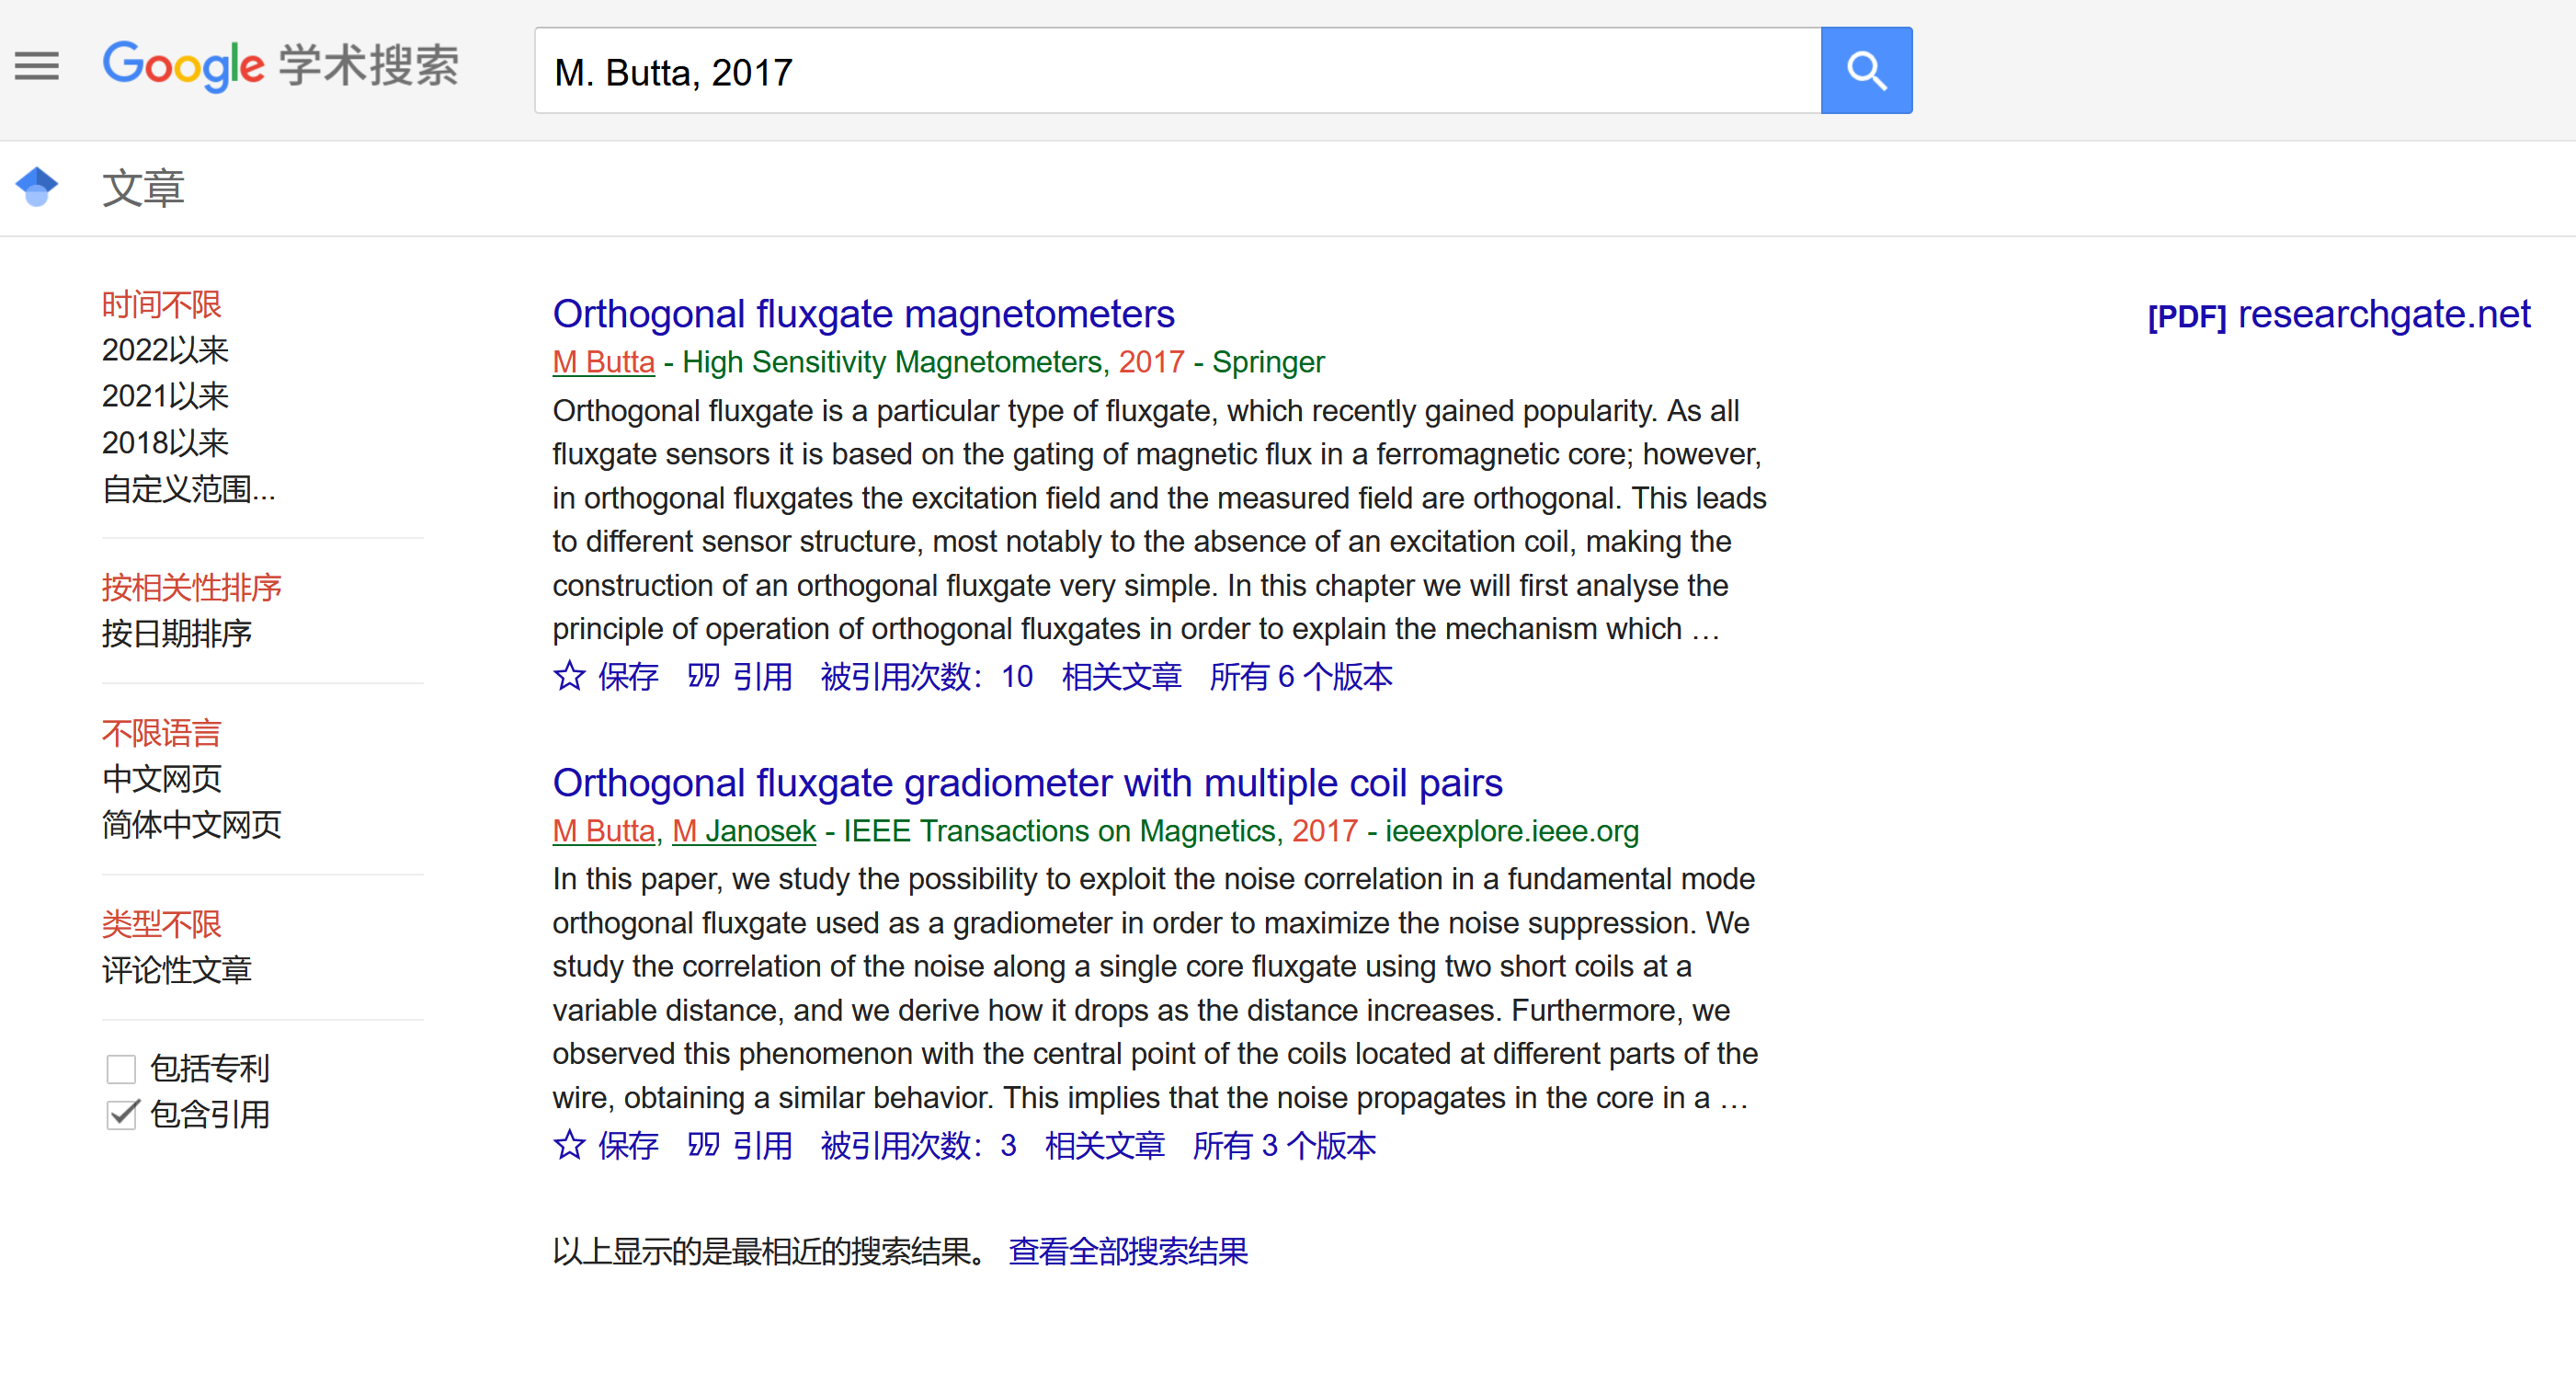
\includegraphics[width=11.5cm]{PICS/Cite1.png}
\caption{在谷歌学术上找到这篇文章}
\end{figure}\par
随后点击“引用”。
\begin{figure}[H]
\label{fig02}
\centering
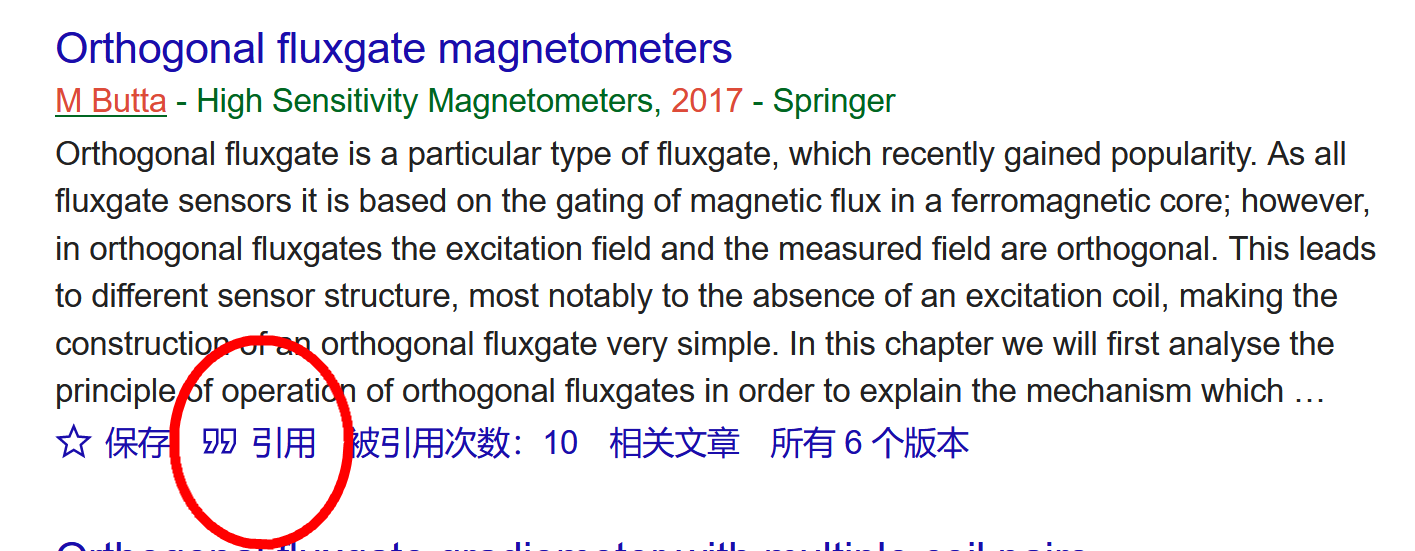
\includegraphics[width=8cm]{PICS/Cite2.png}
\caption{红圈里的引用点击一下}
\end{figure}\par
在弹出窗口里选择“BibTex”。
\begin{figure}[H]
\label{fig03}
\centering
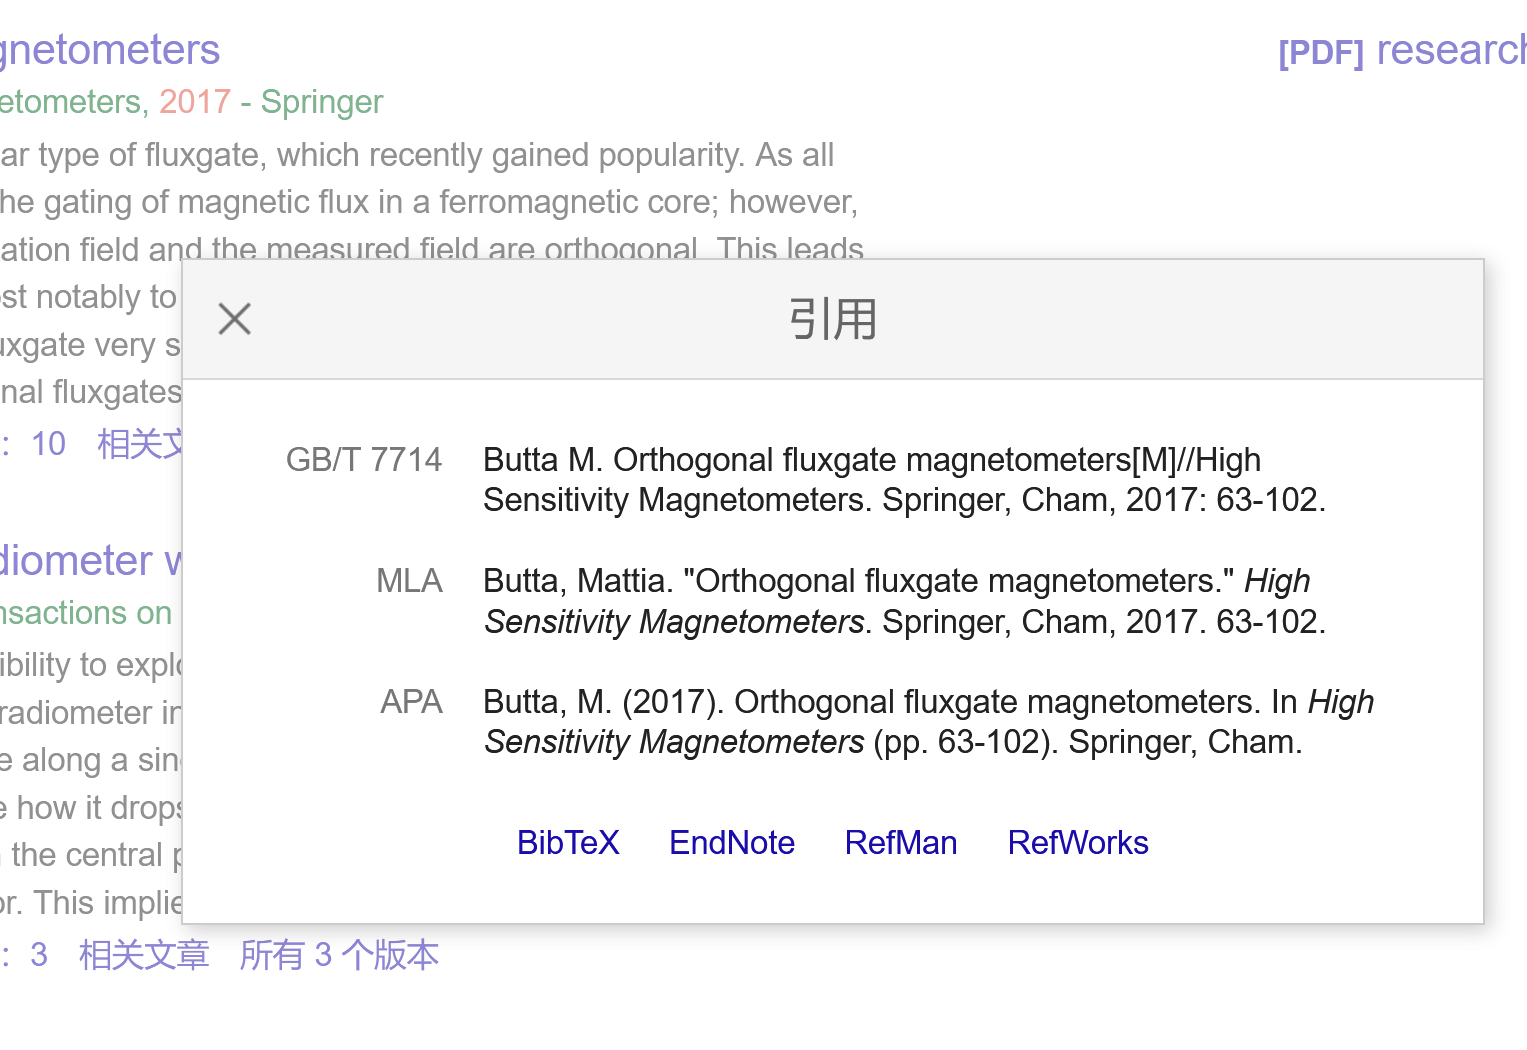
\includegraphics[width=8cm]{PICS/Cite3.png}
\caption{左下角的BibTex}
\end{figure}\par
然后会弹出一个窗口,里面有这样一些内容。
\begin{figure}[H]
\label{fig04}
\centering
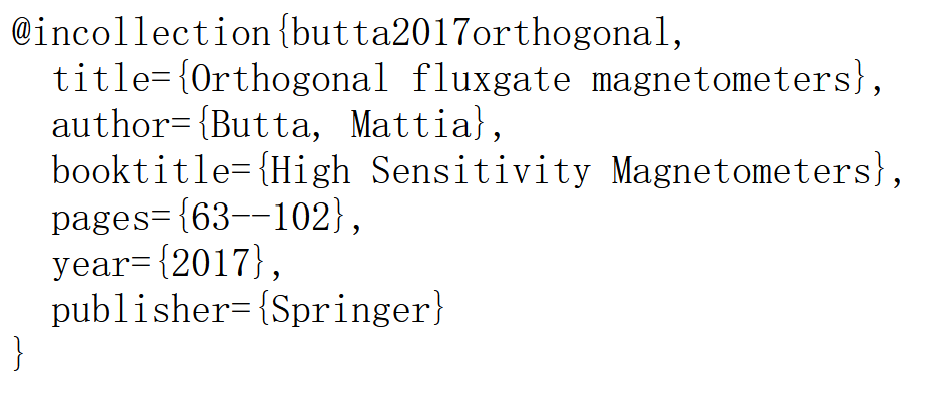
\includegraphics[width=8cm]{PICS/Cite4.png}
\caption{BibTex的全部信息。一般至少包括了题目,作者,年份,杂志(书籍),出版商等。有些还有DOI号,页码,网页链接等。不同的文献类别包含的基本信息也会不同,比如这篇是incollection,属于论文集的一部分。一般的文章是article,还有书籍book。详见教程。}
\end{figure}\par
全选并复制这些内容,粘贴进一个空白的txt文档中,例如\textit{testRef.txt},并另存为\textit{testRef.bib}。值得注意的是,这是一个文本文档,所以编码模式很重要。如果你的参考文献中只有英文,那么可以忽略。但如果你的参考文献中还含有中日韩语,西里尔文,拉丁文,希腊文的话,一定要注意编码模式,ANSI或GB2312可能会导致一系列的报错,尤其是会导致中日韩文出现乱码。另存为的时候一定要注意编码模式设置为UTF-8。具体如何设置请自行百度。
\begin{figure}[H]
\label{fig05}
\centering
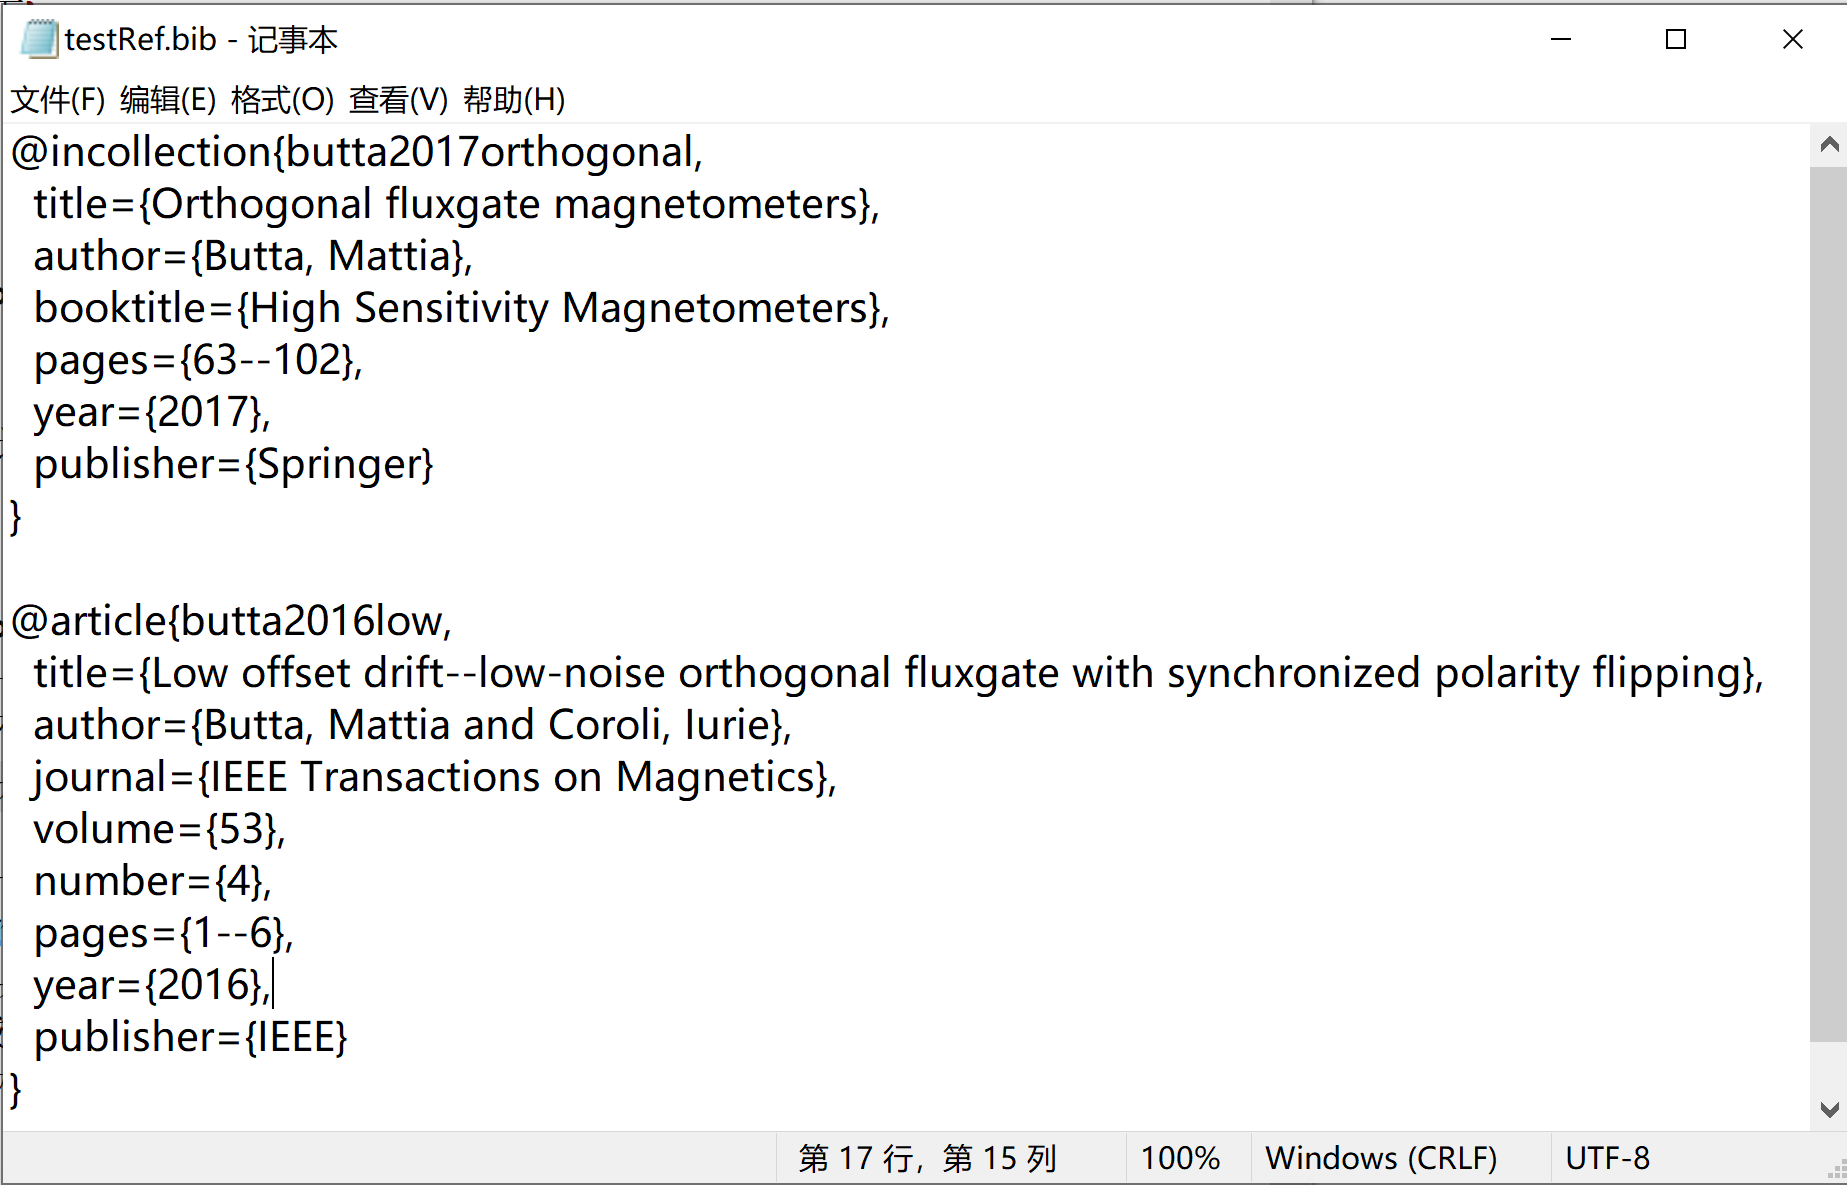
\includegraphics[width=9cm]{PICS/Cite5.png}
\caption{Bib数据库}
\end{figure}\par
注意,可以用一个Bib文件来容纳所有用到的或者没用到的参考文献。没用到的参考文献就算出现在了Bib文件里,如果文章中没有引用,也不会出现在最后生成的论文参考文献列表中。\par
你可以一边写论文,一边把自己用到的参考文献扔进这个库里。也可以从EndNote里批量导出Bib。Bib文件中的顺序无关紧要。另,Bib其实是bibliography的缩写,是参考文献的学名,意为目录学,参考书目,文献学,索引。\par
现在,你只要记忆如图\ref{fig06}红框圈出来的这个关键字,就可以在后面的教程中引用这篇文献了。\par
\begin{figure}[H]
\label{fig06}
\centering
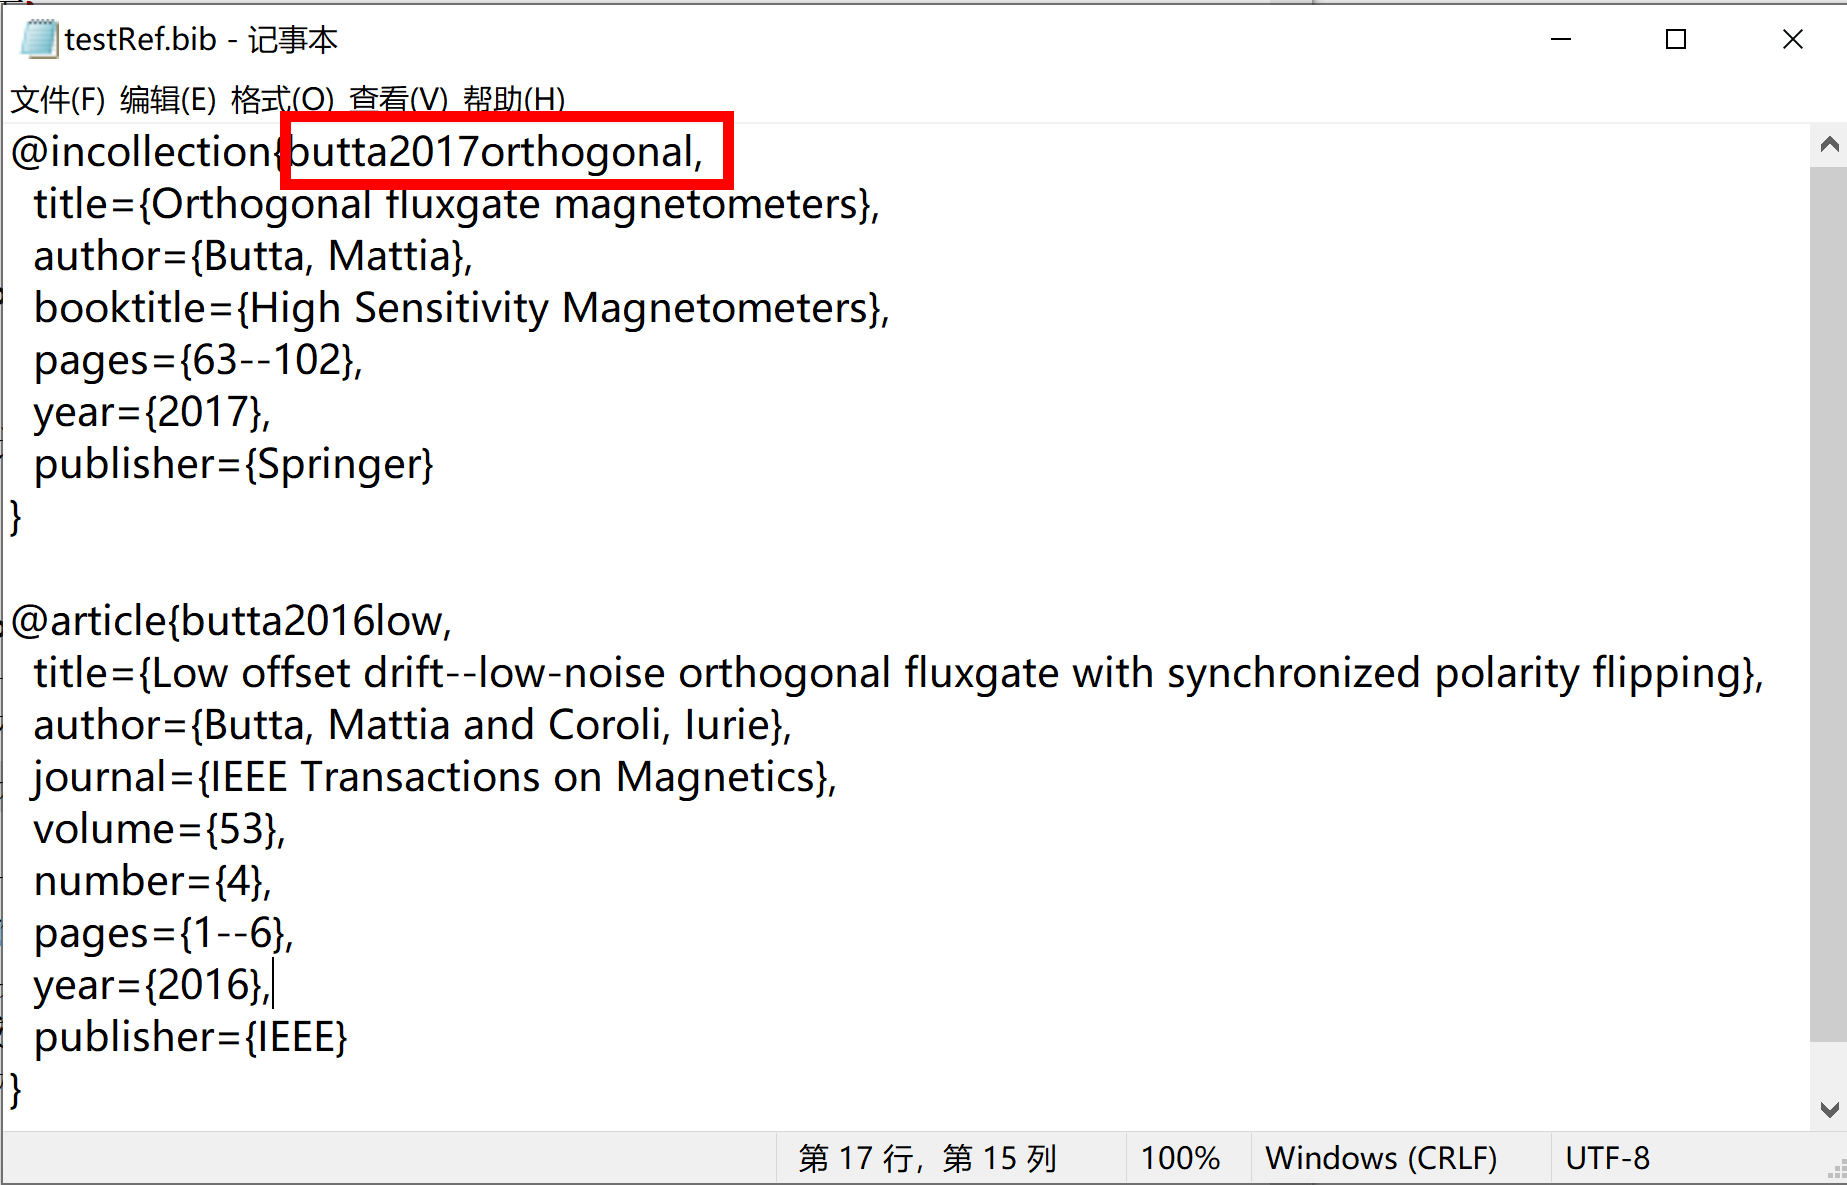
\includegraphics[width=9cm]{PICS/Cite6.png}
\caption{Bib关键字,注意,Bib库里绝不能存在重复的关键字,不然会报错。}
\end{figure}\par
\reposubsec{人名,时间都在括号里的完整引用}
当我们想要获得形如\citep{butta2017orthogonal}这样的参考文献样式,则你只需要在相应的位置使用$\backslash citep\{butta2017orthogonal\}$这个命令标志即可。其中的\textit{butta2017orthogonal}就是我前面说到的参考文献的关键字。只要这个关键字所代表的文献在你的参考文献库中,就可以成功引用。在文中你可以多次引用同一篇文献,参考文献列表只会出现一次。\par
这个命令可以同时写好几篇参考文献,会自动并列放好,例如:\citep{Yuan2020Graphene, butta2017orthogonal},或者同一个作者的多篇文章:\citep{butta2017orthogonal, butta2012orthogonal}。注意,多篇文献的关键字之间用西文的逗号分割,不要用中文逗号!\par
\reposubsec{人名在括号外,时间在括号里的引用}
当我们想要获得形如:\ \ \textit{在非晶磁强计领域,\citet{butta2017orthogonal}做出了重大突破}\ \ 这样的参考文献引用样式时,只需要在相应位置使用$\backslash citet\{butta2017orthogonal\}$这个命令标志即可。注意,这个参考文献样式已经自带了人名,所以你不需要再写一遍人名了。如果有多名作者,名字后面会自动带上et al.。并且显然,同一个作者的多篇文章\citet{butta2017orthogonal, butta2012orthogonal}的形式也可以正确表示。\par
\reposubsec{非引用参考文献}
有些参考文献对于这篇文章很重要,但是你却找不到恰当的地方进行引用,那么你可以考虑非引用参考文献。这种引用形式不会出现在正文中,但却会出现在参考文献列表中。相应的命令是例如:$\backslash nocite\{butta2016low\}$这样的语句。模板中,这样的参考文献统一写在了主文件Report.tex的正文部分最后。\par
\reposubsec{编译注意事项}
仅仅写了这些citep,citet或者nocite的引用项,并不会在文章最后生成引用文献列表。这需要你在需要插入参考文献的位置,添加一句话。$\backslash bibliography\{testRef\}$,注意将testRef修改为你自己的Bib库的名字。这句话放在哪里,就会在那个地方生成参考文献。\par
另外,为了使参考文献的数据库与文中的参考文献链接起来,并生成参考文献列表和交叉引用的链接,我们需要{\Large{\color{red}先跑一遍XeLaTeX编译,然后再跑一遍BibTex编译,然后再连续跑两遍XeLaTeX编译}}。没有别的捷径!